%%%%%%%%%%%%%%%%%%%%%%%%%%%%% Define Article %%%%%%%%%%%%%%%%%%%%%%%%%%%%%%%%%%
\documentclass{article}
%%%%%%%%%%%%%%%%%%%%%%%%%%%%%%%%%%%%%%%%%%%%%%%%%%%%%%%%%%%%%%%%%%%%%%%%%%%%%%%

%%%%%%%%%%%%%%%%%%%%%%%%%%%%% Using Packages %%%%%%%%%%%%%%%%%%%%%%%%%%%%%%%%%%
\usepackage{geometry}
\usepackage{graphicx}
\usepackage{amssymb}
\usepackage{amsmath}
\usepackage{amsthm}
\usepackage{empheq}
\usepackage{mdframed}
\usepackage{booktabs}
\usepackage{lipsum}
\usepackage{graphicx}
\usepackage{color}
\usepackage{psfrag}
\usepackage{pgfplots}
\usepackage{bm}
\usepackage{wrapfig}
\usepackage{hyperref}
\usepackage{url}
\usepackage{float}
\usepackage{pythonhighlight}
\usepackage{listings}
%%%%%%%%%%%%%%%%%%%%%%%%%%%%%%%%%%%%%%%%%%%%%%%%%%%%%%%%%%%%%%%%%%%%%%%%%%%%%%%

% Other Settings

% Listing Settings for Python

\lstset{
    language=Python,
    basicstyle=\ttfamily\small,
    keywordstyle=\color{blue},
    stringstyle=\color{red},
    commentstyle=\color{green},
    morecomment=[l][\color{magenta}]{\#}
}

%%%%%%%%%%%%%%%%%%%%%%%%%% Page Setting %%%%%%%%%%%%%%%%%%%%%%%%%%%%%%%%%%%%%%%
\geometry{a4paper}

%%%%%%%%%%%%%%%%%%%%%%%%%% Define some useful colors %%%%%%%%%%%%%%%%%%%%%%%%%%
\definecolor{ocre}{RGB}{243,102,25}
\definecolor{mygray}{RGB}{243,243,244}
\definecolor{deepGreen}{RGB}{26,111,0}
\definecolor{shallowGreen}{RGB}{235,255,255}
\definecolor{deepBlue}{RGB}{61,124,222}
\definecolor{shallowBlue}{RGB}{235,249,255}
%%%%%%%%%%%%%%%%%%%%%%%%%%%%%%%%%%%%%%%%%%%%%%%%%%%%%%%%%%%%%%%%%%%%%%%%%%%%%%%

%%%%%%%%%%%%%%%%%%%%%%%%%% Define an orangebox command %%%%%%%%%%%%%%%%%%%%%%%%
\newcommand\orangebox[1]{\fcolorbox{ocre}{mygray}{\hspace{1em}#1\hspace{1em}}}
%%%%%%%%%%%%%%%%%%%%%%%%%%%%%%%%%%%%%%%%%%%%%%%%%%%%%%%%%%%%%%%%%%%%%%%%%%%%%%%

%%%%%%%%%%%%%%%%%%%%%%%%%%%% English Environments %%%%%%%%%%%%%%%%%%%%%%%%%%%%%
\newtheoremstyle{mytheoremstyle}{3pt}{3pt}{\normalfont}{0cm}{\rmfamily\bfseries}{}{1em}{{\color{black}\thmname{#1}~\thmnumber{#2}}\thmnote{\,--\,#3}}
\newtheoremstyle{myproblemstyle}{3pt}{3pt}{\normalfont}{0cm}{\rmfamily\bfseries}{}{1em}{{\color{black}\thmname{#1}~\thmnumber{#2}}\thmnote{\,--\,#3}}
\theoremstyle{mytheoremstyle}
\newmdtheoremenv[linewidth=1pt,backgroundcolor=shallowGreen,linecolor=deepGreen,leftmargin=0pt,innerleftmargin=20pt,innerrightmargin=20pt,]{theorem}{Theorem}[section]
\theoremstyle{mytheoremstyle}
\newmdtheoremenv[linewidth=1pt,backgroundcolor=shallowBlue,linecolor=deepBlue,leftmargin=0pt,innerleftmargin=20pt,innerrightmargin=20pt,]{definition}{Definition}[section]
\theoremstyle{myproblemstyle}
\newmdtheoremenv[linecolor=black,leftmargin=0pt,innerleftmargin=10pt,innerrightmargin=10pt,]{problem}{Problem}[section]
%%%%%%%%%%%%%%%%%%%%%%%%%%%%%%%%%%%%%%%%%%%%%%%%%%%%%%%%%%%%%%%%%%%%%%%%%%%%%%%

%%%%%%%%%%%%%%%%%%%%%%%%%%%%%%% Plotting Settings %%%%%%%%%%%%%%%%%%%%%%%%%%%%%
\usepgfplotslibrary{colorbrewer}
\pgfplotsset{width=8cm,compat=1.9}
%%%%%%%%%%%%%%%%%%%%%%%%%%%%%%%%%%%%%%%%%%%%%%%%%%%%%%%%%%%%%%%%%%%%%%%%%%%%%%%

%%%%%%%%%%%%%%%%%%%%%%%%%%%%%%% Title & Author %%%%%%%%%%%%%%%%%%%%%%%%%%%%%%%%
\title{Coding with AI Assignment}
\author{Ali Muhammad Asad \\ aa07190}
\date{} %Leave uncommented if u want automatic date which is done through maketitle, else u can uncomment this and type anything else u want over here - not necessary to enter a date over here
%%%%%%%%%%%%%%%%%%%%%%%%%%%%%%%%%%%%%%%%%%%%%%%%%%%%%%%%%%%%%%%%%%%%%%%%%%%%%%%

\begin{document}
    \maketitle

\subsection*{1. Problem Statement}
\textbf{Finding Median from a Data Stream:} The median is the middle value in an ordered integer list. If the size of the list is even, there is no middle value, and the median is the mean of the two middle values. So the problem was to continously find the median given an array of integers, and a stream of instructions, such as ``MedianFinder'', ``addNum'', and ``findMedian'', where ``addNum'' adds a number to the array, and ``findMedian'' returns the median of the array, while ``MedianFinder'' initializes the MedianFinder object. 

\noindent The image below describes an example input, output, and its explanation.
\begin{figure}[H]
    \centering
    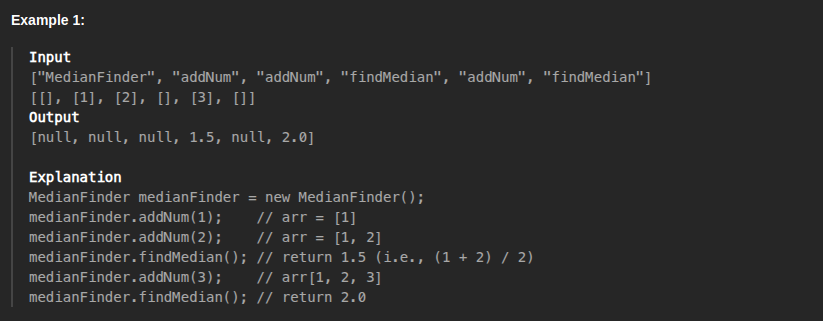
\includegraphics[width=\textwidth]{median_finder.png}
    % 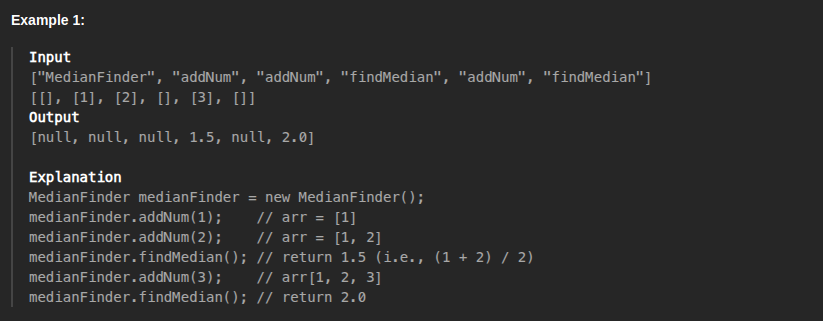
\includegraphics[width=0.5\textwidth]{median_finder.png}
\end{figure}

\subsection*{2. My Solution}
If we tackle this problem using the brute force approach, we can simply add the number to the array, sort the array, and then find the median. However, this approach is not efficient, as the time complexity of sorting the array is $O(n\log n)$, where $n$ is the number of elements in the array, and we do this each time a new element is added which is not efficient and would bring the time complexity to $O(n^2\log n)$.

Thus, I approached this problem by maintaining two heaps; a max heap (which would store the larger half of the array), and a min heap (which would store the smaller half of the array). Since the median is the middle value, by maintaining two heaps, we ensure that the median is always at the top of the heaps; if the total number of elements is odd, then the median of the two elements is on top of the max heap, and if the total number of elements is even, then the median is the average of the top elements of the two heaps. 

This approach is efficient as the time complexity of adding an element to the heap is $O(\log n)$, and since we add $n$ elements, the time complexity of the entire operation is $O(n\log n)$, as taking the top element of the heap is $O(1)$. Further, the space complexity of this approach is $O(n)$, as we are storing $n$ elements in the heap. 

My solution passed all the test cases, ran in 424ms, beating 72.76\% of the submissions, while taking a memory of 35.44 MB. 

\subsection*{3. LLM 1 - ChatGPT 4o}
I passed the entire prompt on Leetcode to ChatGPT 4o and then ran its provided code to see if it could solve the problem. ChatGPT had the same idea of maintaining two heaps, and its code was similar to mine, however, it had more conditional checks than mine hence took more time than mine to run. 

ChatGPT's code was more easier to follow through since it also provided comments at every step, and made it more readable. Since the approach is the same, the time complexity of ChatGPT's code is also $O(n\log n)$, and the space complexity is $O(n)$.

GPT's solution passed all the test cases, ran in 490ms, beating 42.99\% of the submissions, while taking a memory of 35.58 MB.

\subsection*{4. LLM 2 - Claude 3.5 Sonnet}
I passed the entire prompt on Leetcode to Claude 3.5 Sonnet and then ran its provided code to see if it could solve the problem. Claude also had the same idea of maintaining two heaps, and its code was similar to mine, however, it had more conditional checks than mine hence took more time than mine to run.

Claude's code was more easier to follow through since it also provided comments at every step, and made it more readable. Since the approach is the same, the time complexity of Claude's code is also $O(n\log n)$, and the space complexity is $O(n)$.

Claude's solution passed all the test cases, ran in 490ms, beating 42.99\% of the submissions, while taking a memory of 35.58 MB. It solution was similar to ChatGPT's solution, and also ran in the same time and memory.

\subsection*{5. Comparison and Analysis}

My solution ran the fastest, beating both ChatGPT and Claude, while taking the same memory as Claude. The reason for this could be that my code had less conditional checks than ChatGPT and Claude, and was more concise. However, considering readability and understandability, ChatGPT and Claude's code was more readable and understandable than mine, as they provided comments at every step, and made the code more readable.

\subsection*{6. Reflection}

The LLMs were able to solve the problem efficiently, and their solutions were similar to mine, however, they had more conditional checks than mine, which made their code less efficient. However, their code was more readable and understandable than mine, as they provided comments at every step, and made the code more readable. I think that LLMs can complement human problem-solving by providing a different perspective to the problem, and can challenge human problem-solving by providing a more efficient solution than the human, or by providing a more readable and understandable solution than the human.

\end{document}